\documentclass[../thesis.tex]{subfiles}

\graphicspath{{../fig/}}

\begin{document}

\chapter{Experimental Setup}

\section{Laser Light production}

The laser light used in the experiment is a monochromatic laser radiation tuned to the transition of the chosen atomic species. In this experiment sodium is the atomic source, as for all the alkali atoms, important transitions are given by the only electron present in the outer shell. The ground state of the external electron is the $^2$S$_{1/2}$, by spin-orbit interaction with the nuclear spin I $= 3/2$, it is split into the F $=1$ and F $=2$ hyperfine levels.
From the level $^2$S$_{1/2}$ transitions are allowed to the states $^2$P$_{1/2}$ and $^2$P$_{3/2}$, called respectively the D1 and D2 line.\\

\begin{figure}[!htb]
\centering
\includegraphics[scale=1]{d2_levstr.pdf}
\caption{Hyperfine level structure of sodium D2 line, with relative strength of each transition and energy spacing in frequency units.}
\label{fig:d2line}
\end{figure}

To obtain an efficient cooling mechanism a closed transition is necessary, in the case of sodium a good closed transition is found on the D2 line, between the F $=2$ and the F$^\prime =3$ hyperfine sublevels, corresponding to a wavelength of 589 nm. Still a repump beam is needed, tuned on the transition F $=1 \rightarrow $F$^\prime =2$, to close the loop with the cooling transition, since the electron can decay from F$^\prime =2$ to F $=1$ due to off-resonance excitations.\\
The laser light is generated by a system composed by diode lasers, amplifiers and doubling cavities. The diode lasers provide an ease and flexible solution for the production of laser radiation, but they cannot reach directly the optical wavelength needed for sodium. The solution is to start from an infrared laser diode at the wavelength of 1178 nm, which is the double of the one needed for the sodium, using it as master laser for an amplifier. The laser radiation of the diode is easily amplified by a Raman fiber amplifier and then the frequency is doubled using a non-linear crystal placed in a resonant optical cavity.\\

The master source is composed by an home-made external cavity diode laser (ECDL) in Littrow configuration, based on the design proposed by Ricci et all.(1995)\citet{Ricci95}. The active medium is a diode with InAs quantum dots on a GaAs substrate (INNOLUME GC-1178-TO-200), with single transverse mode and an anti-reflection coating on the output facet. The light of the diode is collimated using an aspheric lens (THORLABS C340TME-C) on a reflective holographic grating for visible wavelengths with 1200 lines per mm (THORLABS GH13-12V). The length of the external cavity is 15 mm, in this way the free spectral range is of the order $\sim$ 10 GHz. The wavelength is tuned roughly with the horizontal screw that fixes the grating, the emission is optimized with the vertical screw and through the control of the current source and the TEC controller. A piezoelectric crystal finely-tune the position of the grating changing the length of the cavity.\\

\begin{figure}[!htb]
\centering
\includegraphics[scale=1]{laser_ricci.pdf}
\caption{Schematic of the ECDL setup taken from the original article of Ricci et all.(1995)\citet{Ricci95}, similar to the design of the master laser.}
\label{fig:mastlas}
\end{figure}

The amplifier of the master source is a Raman fiber amplifier (MPB RFA-SF-SERIES) pumped by an Ytterbium fiber laser. In the amplifier are injected $\sim$ 10 mW of power from the master laser and the amplifier returns an output of 6-7 W on a single laser mode, maintaining polarization and spectral properties of the input beam.\\

The infrared radiation is then frequency doubled through \textit{second harmonic generation}, implemented with an external cavity with a non-linear crystal (<<Inserire reference>>). The crystal is made of LiB$_3$O$_5$ and it is long 15 mm. The cavity is a bow-tie cavity with a length $\sim$ 300 mm and a finesse of about 150. The temperature of the crystal is stabilized by a TEC controller and it is setted at <<Controllare valore temperatura>>. The output power from the cavity is around 3.5 W of 589 nm laser light.\\

The master laser is stabilized performing FM saturated absorption spectroscopy on a sodium vapour-cell. The spectroscopic signal gives a direct frequency reference to the D2 and D1 line, such signal is converted into an error signal through a lock in demodulation and it is passed to a PID controller, which close the feedback loop. The feedback circuit acts on the piezo transducer of the master cavity keeping the output frequency locked to the chosen transition.\\
The output of the doubling cavity is split into several beams controlled independently in power and frequency. The power control is performed with the combination of half-wave plates and polarizing beam splitters (PBS). Frequency and amplitude control is realized in real-time with the help of \textit{acousto-optical modulators} (AOM) and \textit{electro-optical modulators} (EOM), in this way the frequency of the beam can be detuned from the locking frequency. Each beam is injected into an optical fiber that preserves the polarization of the input beam (Schäfter\&Kirchhoff PMC-630-4.5-NA011-3-APC-900-P) and transmitted to the main experiment table. For a schematic of the of the oprical setup for the D2 cooling and probing see Fig. \ref{fig:d2_table}.\\

\begin{figure}[!htb]
\centering
\includegraphics[scale=1]{d2_schematic.pdf}
\caption{Schematic of the optical setup generating the laser beams for the sodium laser cooling apparatus. The beams are split from the main beam through half-wave plates and PBS. Collimating optics and the mechanical shutters are omitted. Each AOM reports its central operative frequency and the sign of the first diffraction order on which the AOM is aligned.}
\label{fig:d2_table}
\end{figure}

The setup is reproduced twice, one setup is locked on the F=2$\rightarrow$F$^\prime$=3 transition, it is used to produce the cooling light, the repumper light and the probe light. The second setup is used to lock on the D1 transition, for a schematic of the D1 setup see Fig. \ref{fig:d1_table}.

\begin{figure}[!htb]
\centering
\includegraphics[scale=1.2]{d1_schematic.pdf}
\caption{Schematic of the optical setup generating the laser beams for the phase imprint. The beams are split from the main beam through half-wave plates and PBS. Collimating optics and the mechanical shutters are omitted. Each AOM reports its central operative frequency and the sign of the first diffraction order on which the AOM is aligned.}
\label{fig:d1_table}
\end{figure}
 

\section{Atomic Source}

The atomic source is a given by a piece of sodium who it is heated at the temperature of 240\degree C and it evaporates and diffuse in the vacuum chamber, this is the primary source. The vacuum chamber is composed by two parts held at different pressure and connected by a differential pumping (DP) channel. The first region is held at high vacuum (HV: 10$^{-10}$ to 10$^{-9}$ mbar), this region contains the crucible with the sodium sample.\\
The steps to be performed before sending the sodium into the ultra-high vacuum (UHV: $\leq$ 10$^{-10}$ mbar) region of the chamber have been inspired by the design proposed for lithium by Tiecke et all.\cite{Tiecke09}. An additional feature to the setup has been added by Lamporesi et all.\cite{Lamporesi13}, introducing a Zeeman slower stage integrated in the 2D-MOT that slows down the atoms coming from the primary source.\\
A vertical laser beam directed toward the sodium oven provide a Zeeman slower stage, exploiting the tails of the 2D-MOT magnetic field, releasing an \textit{increasing-field Zeeman slower} configuration. This design provide a slowing-system compact, since it is built-in into the 2D-MOT, and improves the loading rate of the 2D-MOT pushing more atoms in the captur range of the trap.\\
The 2D-MOT is placed about 10 cm above the oven and it is composed by two orthogonal retro-reflected laser beams and a set of eight stacks of permanent magnets to create the necessary quadrupole field.\\
To transport the captured atoms into the UHV region of the chamber a laser beam perpendicular to the 2D-MOT plane pushes the atoms into the DP channel and then the atoms are recaptured by a 3D-MOT placed in a quartz cell.\\

This design has many advantages:
\begin{itemize}
\item Only pushed atoms can pass the DP channel and reach the 3D-MOT. This avoid the possibility of collisions with hot atoms coming from the oven, which helps to keep the science chamber clean and improve the condensate lifetime. Furthermore the flux of atom can be controlled by the modulation of the push beam, in order to suppress the flux while the main experiment is running;
\item The collimation of the beam is given by the 2D-MOT and the divergence of the beam is given by the transverse temperature. This produce a reduction of the losses since extra diaphragms are not needed for further collimation. The position of the 2D-MOT near the DP channel reduce the limitations of the divergence;
\item The apparatus is also suitable to use different atomic species, due to the radial symmetry of the 2D-MOT it can be transversely loaded from different sources. The setup is already set for the use with potassium from a vapour-cell MOT and strontium with a strontium oven already present. The cooling lights for the different atomic species are overlapped with dichroic mirrors on the 2D-MOT beams directions. 
\end{itemize}

\newpage

\begin{figure}[!htb]
\centering
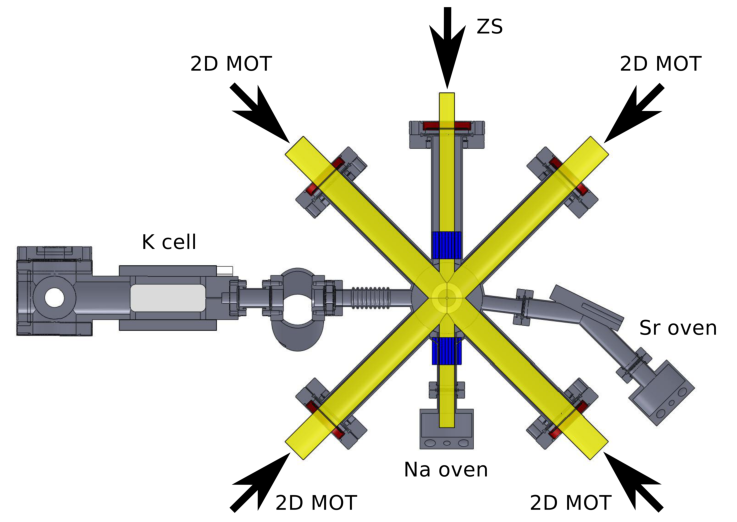
\includegraphics[scale=0.85]{2d_MOT.pdf}
\caption{Front view of the 2D-MOT.}
\label{fig:2d_front}
\end{figure}

\begin{figure}[!htb]
\centering
\includegraphics[scale=0.85]{quartz_cell.pdf}
\caption{Schematic model of the quartz cell, including the directions of the 3D-MOT laser beams. The cell has dimensions 35 mm $\times$ 80 mm $\times$ 60 mm. The shape is of a polyhedron with six 4 mm thick flat surfaces, the largest four of them have been treated with a broadband anti-reflective coating on the outer surfaces to improve optical performances, with a reflectivity R$\sim$0.5\% over the spectral range 530 $\divisionsymbol$ 1100 nm.}
\label{fig:qt_cell}
\end{figure}

\begin{figure}[!htb]
\centering
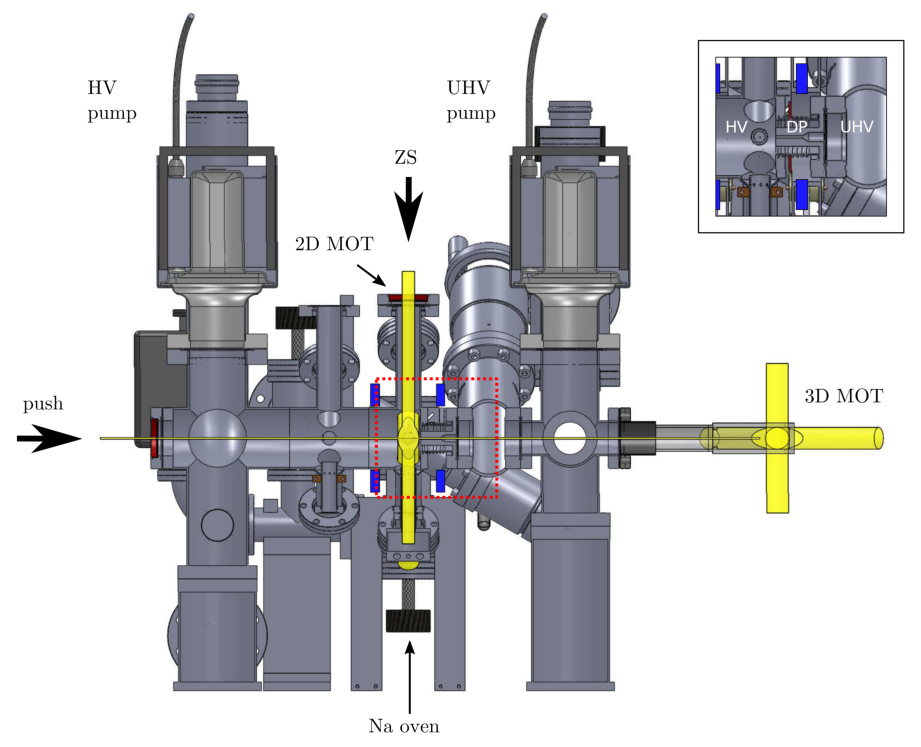
\includegraphics[scale=1]{side_schematic.pdf}
\caption{Side view of the sodium source. The laser beams positions are underlined by the yellow areas, in the figure are shown the 2D-MOT and the 3D-MOT configurations and the thin horizontal one is the push beam. The four stacks of magnets for the 2D-MOT and the Zeeman slower are reported in blue. In the inset there is a zoom of the differential pumping channel, positioned in the red rectangle, which separates the HV from the UHV region.}
\label{fig:side}
\end{figure}


\section{MOT and Magnetic Trap}

Around the quartz cell there is a system of coils, Fig. \ref{fig:sch_mt}, which provide the trapping magnetic fields requireb by the different configurations:

\begin{itemize}
\item \textbf{MOT}: during the 3D-MOT, a quadrupole field is provided by the two horizontal coils, in which the current flow in anti-Helmoltz configuration;
\item \textbf{MT}: the pinch coil is added in series to the quadrupole and generates a bias and curvature field along \textit{z}, resulting in a "three-coils" Ioffe-Pritchard magnetic trap;
\item \textbf{MTC}: the two compensation coils are added in series in Helmoltz configuration, to allow tuning of the bias term in the trap and compensation of gravitational field;
\item \textbf{LM$\uparrow$}: a magnetic levitation is obtained turning-on only the lower quadrupole coil and is used to compensate gravity during the long time-of-flight imaging.
\end{itemize}

When the atoms are in the magnetic trap, the maximum current flowing in the coils is 200 A at the start of the evaporative cooling procedure, it is ramped down to 100 A or 50 A to set the potential in which BEC is achieved. The coils are made with thin copper tubes in which flow at high pressure cold water to dissipate the heat produced during the operations.\\

\begin{figure}[!htb]
\centering
\includegraphics[scale=1]{schematic_mt.pdf}
\caption{(a) A scheme of the magnetic IP trap configuration, with the two horizontal quadrupole coils (Q$_{up}$,Q$_{dw}$), the smaller pinch coil in the middle (P) and the farther compensation (C$_1$, C$_2$). (b) Top view of the quartz cell positioning inside the coil system; the laser beams are show in yellow and show the access of the push beam and the cooling light.}
\label{fig:sch_mt}
\end{figure}


\section{Electronic Controls}

The experiment need a precise control in the time sequence in which the operations are performed. In this case, such control is achieved through a digital software-hardware interface, developed by prof. Marco Prevedelli from University of Bologna and then adapted to the needs of the of the setup.\\
The user interface is a custom made software developed in Python, which defines in a tabular form the temporal sequence of actions to be performed. The software convert the table and send it via USB cables to the interface motherboards, one for each table. The motherboard mount a XILINX SPARTAN XC3S250E FPGA with a clock at 10 MHz, synchronized by an ARDUINO who provide the signal who starts the execution of the actions. The FPGAs manage the list of actions in real-time, communicating through a 24-bit parallel bus the action commands in the temporal sequence given before. The bus is connected to the device controller-boards to which different addresses are assigned: controller boards read only the actions assigned to their address and the actions are updated with a strobe pulse at the correct time.\\
Devices are controlled with three types of commands:

\begin{itemize}
\item RF inputs for the AOMs and the evaporative cooling are generated by Direct Digital Synthesizers (DDS) boards mounting an ANALOG DEVICES AD9958 dual channel chip, these devices are directly connected to the communication bus and allow to synthesize AC voltage signals whose frequency, amplitude and phase can be tuned easily;
\item devices like mechanical shutters, relais, some IGBTs and camera triggers are driven by logical signals delivered by a TTL driver connected to the communication bus;
\item two IGBTs are driven by DAC boards to permit analogical control of their state, such boards are also used to control the power supplies for the coils.
\end{itemize}

The maximal temporal resolution of the system is of 100 ns with a maximum update rate of 2.5 MHz.

\begin{figure}[!htb]
\centering
\includegraphics[scale=1]{circ_mot.pdf}
\caption{Schematic of the electric circuit of the magnetic trap. The circuit allows to switch between the different magnetic field configurations: quadrupole, trap and levitation.}
\label{fig:circ_mot}
\end{figure}


\section{Dipole Trap}

A dipole trap has been implemented in order to trap atoms in states which the magnetic potential could not trap. The trap is constituted by two crossed beams of infrared light with a wavelength of 1064 nm, far detuned from any optical transition of the sodium. The radiation needed to produce the optical dipole trap is provided by a Mephisto MOPA Laser System, the laser emits at a centre wavelength 1064 nm on a single longitudinal mode with spectral linewidth of about 1 kHz. The laser is operated at a current I = 45 A, which corresponds to an output power of 30 W.\\
The light is sent to the atoms through photonic crystal optical fibers, the optical fibers are NKT Photonic Single-Mode polarization maintaining fibers with a length of 5 m (LMA-PM-10 and LMA-PM-15) and can withstand powers to 15 W at 1064 nm. The input collimator are Schäfter\&Kirchhoff 60-FC-SMA-T-23-A18-03, with a focal length of 18 mm, a numerical aperture NA=0.15, and a coating for a range of wavelengths between 1050 nm to 1550 nm. At the output no collimators are used, but the beam are collimated by a two lenses one with focal length with 50 mm and the other with focal length 30 mm.\\
A frequency doubling crystal is placed along the path and produces green light previously used to create a blue-detuned optical potential. The green light is filtered out by an Edmund Cold Mirror.\\

\subsection{Power Stabilization and Control}

The stabilization and control of the laser signal has been achieved through two AOMs (CRYSTAL THECNOLOGY AOM 3110-197) placed before the fiber injection of the beams and a feedback loop, as shown in Figure<<inserire figura>>. The signal of the laser is sampled, at the output of the high power fibers, using a wedge (THORLABS PS811-C) with 4\degree angle with a reflectance of $\sim$ 0.25 \% at a wavelength of 1064nm. The sampled signal is sent to a photodiode (PDA 100A-EC 340-1100 nm), in front of the two photodiodes two optical density have been placed to regulate the light power impinging on the sensor. The signal of the photodiode is sent to a PID controller (SIM 960 ANALOG PID CONTROLLER) as \textit{measure} signal. The \textit{setpoint} signal for the PID is provided by a DAC board, which permits to perform easily the temporal control of the dipole beams. The \textit{output} signal of the PID is inverted and amplified four times (SIM954 300MHz), then it is sent to a mixer (MINI-CIRCUITS ZLW-1-1+ 0.1-500 MHz) which multiply it with the RF signal from the DDS and send it to the AOMs. In this way the diffraction efficiency of the AOMs is modulated to control the signal of the photodiodes.\\
The PID control and stabilization is made through a proportional circuit and an integral circuit. The two parameters has been chosen using the Ziegler-Nichols closed loop tuning.


\section{Phase Imprint Setup}

The laser light needed to implement the \textit{phase imprint} is provided by the D1 setup and an optical fiber transport it to the main experiment bench. <<Inserire parte tipo fibra e collimazione con valore waist>> The gaussian intensity profile is shadowed using a knife edge, to produce a step variation of it. The image of the knife edge is projected on the atoms using a telescope with magnification equal to one. The telescope is composed by two achromatic lenses with focal length equal to 100 mm (THORLABS AC254-100-A).\\
The resolution power of the telescope is given by the diffraction limit of the two lenses. The diffraction limit is given by the formula 1.22$\lambda$/NA, where NA is the numerical aperture of the lens. The numerical aperture is calculated from the diameter and the focus length of the lens as NA = diameter/f. In this setup the lenses that project the image of the knife edge on the atoms have a diameter of 2.5 cm and a focal length of 100 mm, then the diffraction limit is 2.87 $\mu$m. Therefore the minimum extinction length should be equal to the diffraction limit of the lenses, but it is much more. The greater diffraction limit is given by the fact that the lenses are not as thin as the condition for the calculation requests.  To correct partially the problem the use of achromatic lenses is necessary, they resolve better the image of the knife edge on the atoms, reducing the diffraction limit to a value of 3.6 $\mu$m and correct possible aberrations due to the position of the beam on the lenses.\\
The knife edge has been mounted on a translation stage to tune finely the blade on the lens' focus.\\

The alignment on the atoms has been done mounting a setup to look at the condensate from the bottom. The setup is composed by two lenses with focal length of 150 mm and a camera (STINGRAY F-201). The magnification of the telescope is not equal to one since the two lenses are placed the first one at 12.5 cm from the atoms, the second one at 28 cm from the first one and the camera is placed at 15 cm from the second lens. In this configuration the magnification of the telescope is M $\sim$ 1.3. The camera has been mounted on a translation stage and the image has been putted on focus minimizing the radial width of the condensate from in-situ imaging. In Figure<<inserire figura>> is reported the graphic of the radial width of the condensate in function of the relative position of the camera on the translation stage.\\

The switching of the phase imprint beam is operated using the two AOMs present before the fiber. The control of the two AOMs is performed through the modulation of the amplitude of the radio-frequency drive signal, with this the efficiency of the AOMs can be manipulated. Setting to zero the drive signal the efficiency drops to zero and there is no more light injected into the fiber. The control of the signal amplitude is not performed by the DDS, due to the response time to a command of 30 $\mu$s, but the signal from the DDS is multiplied through a mixer (MINI-CIRCUITS ZLW-1-1+ 0.1-500 MHz) with an analogic signal from a TTL, which permit the control of the signal with a resolution of 100 ns and a maximum update rate of 2.5 MHz.\\


\end{document}